\documentclass{beamer}
\usepackage{tikz}
\usepackage{pgf}
\usepackage{listings}
\usepackage{inputenc}
\usetikzlibrary{shapes,arrows}
\usetikzlibrary{automata,positioning}     
% \usepackage{beamerthemesplit} // Activate for custom appearance

\title{OTA Updates for an IOT Security Device}
\author{Aneesh Malhotra, Ryan Thomas, Sohail Iqbal, Gerson Dalton, Mohammad Nur}
\date{\today}

\titlegraphic{\vspace*{-1cm}\hspace*{9cm}~%				%% puts title graphic only on first page
   
\includegraphics[width=2cm]{logoj.jpg}
}


\usetheme{Singapore}
\usepackage{siunitx}
\begin{document}

\frame{\titlepage}

\section[Outline]{}
\frame{\tableofcontents}

\section{Introduction of Problem}
\subsection{Motivation}
\frame
{
  \frametitle{Motivation}
  
  \begin{itemize}
  \item Wireless sensor network are becoming increasingly popular for both industrial and commercial use.
  \item FPGA's can be used to enhance security in wireless sensor networks by implementing a cryptographic exchange between wireless nodes in a network.  \cite{sen_security_2013} \cite{g_elliptic_2016}
  \item Advancements in network attacks, however, could potentially leave these systems vulnerable. 
  \item In the event the system is compromised it may be necessary to implement a firmware update.
  \item Over-the-air updates are those that occur wirelessly, and are easily distributed.
  \end{itemize}
}

\subsection{Current System} 
\frame{
\frametitle{Current System}

\begin{figure}[!ht]
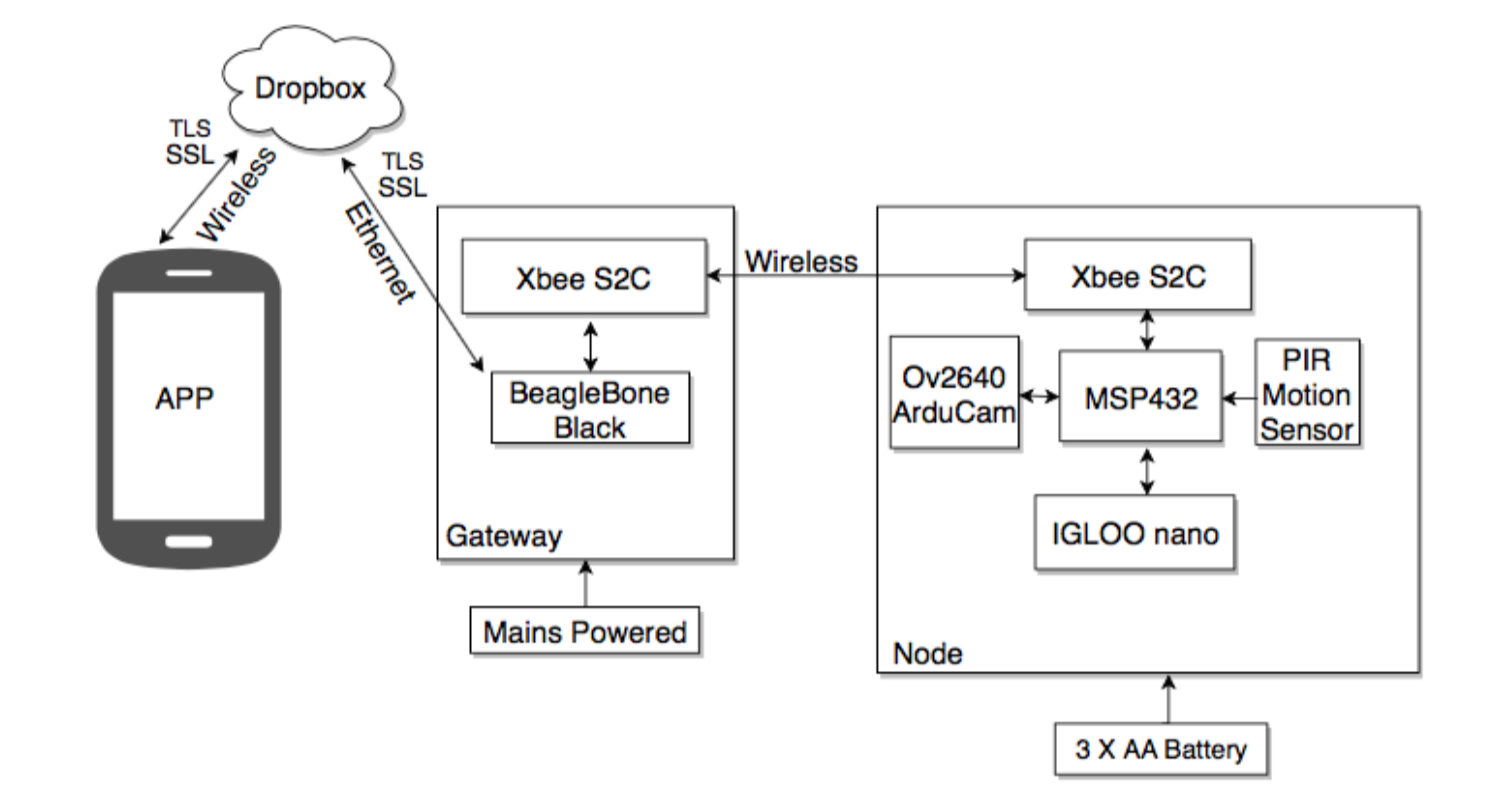
\includegraphics[scale = 0.33]{schematic1.png}
\caption{Top Level Design of IoT Security Device}
\end{figure}
}
\frame{
\frametitle{Current System}

\begin{figure}[!ht]
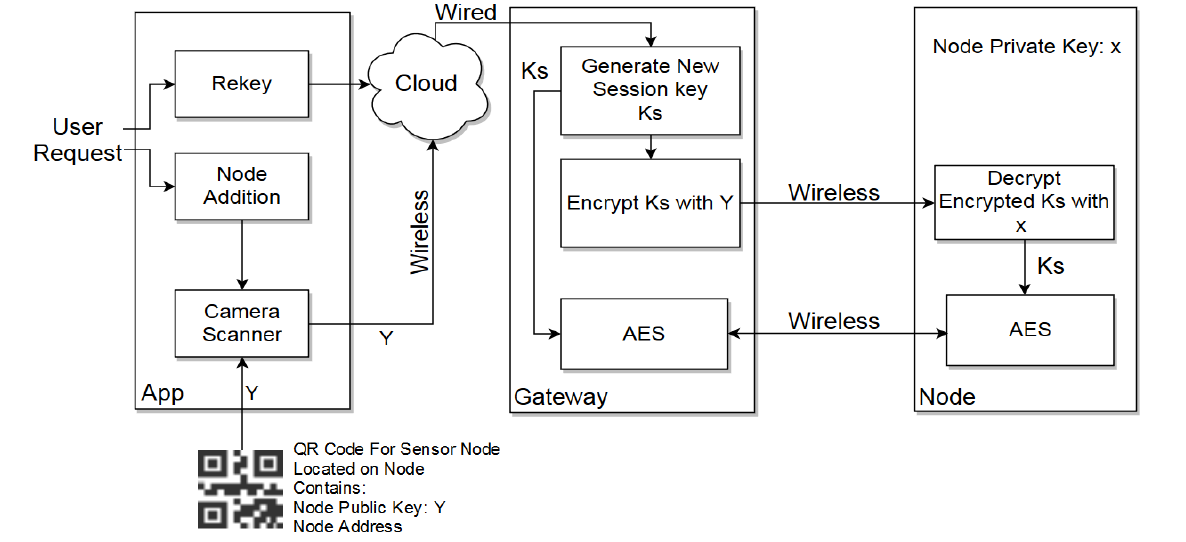
\includegraphics[scale = 0.4]{functional.png}
\caption{Functional Diagram of IoT Security Device}
\end{figure}
}

\frame{
\frametitle{Problems}

\begin{itemize}
\item This node consists of both a microcontroller and an FPGA, both of which need to be updated.
\item We need to be able to distribute an update to the user.
\item  Gateway must be capable of receiving an update and pushing it to the node.
\item The node must be capable of receiving an update from the Gateway and reprogramming itself.
\end{itemize}
}

\section{Solution}

\frame{
\frametitle{Solution}
\begin{columns}[T] % align columns
\begin{column}{.48\textwidth}
\begin{center}
\textbf{Gateway}
\end{center}
\begin{itemize}
\item Requests update from an external server, removing the need for Dropbox and increasing performance.
\item Parses the update and sends bootloader commands to MSP432 corresponding to blocks of memory to be programmed
\vspace{4cm}
\end{itemize}
\end{column}%
\hfill%
\begin{column}{.48\textwidth}
\begin{center}
\textbf{Node}
\end{center}
\begin{itemize}
\item MSP432 will accept the update from the XBee
\item The MSP432 will enter a bootloader and use instructions to update itself
\item The MSP432 will interface to the FPGA via JTAG, and have a STAPL player for programming the FPGA. 
\vspace{4cm}
\end{itemize}

\end{column}%
\end{columns}
}

\section{System Design}

\frame{
\frametitle{System Design}
\begin{figure}[!ht]
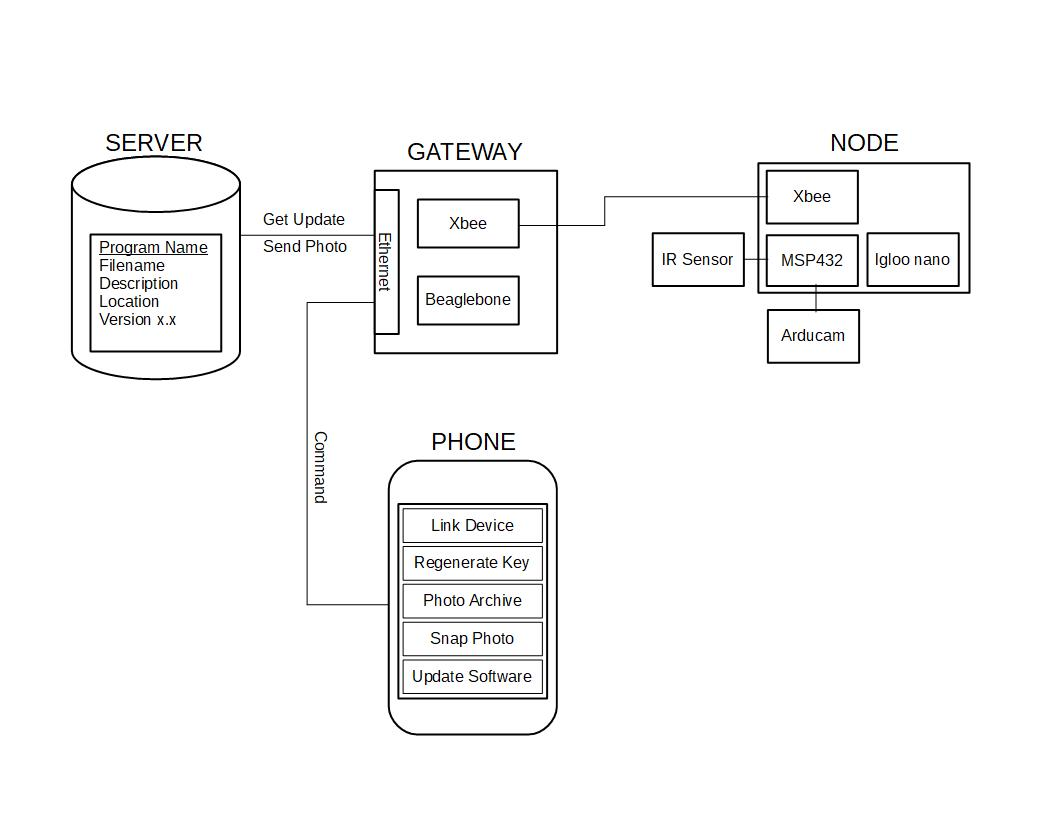
\includegraphics[scale = 0.3]{BlockDiagram.jpg}
\caption{Top Level Design of OTA System with Server}
\end{figure}
}

\frame{
\frametitle{Functional Diagram for Update}

\begin{figure}[!ht]
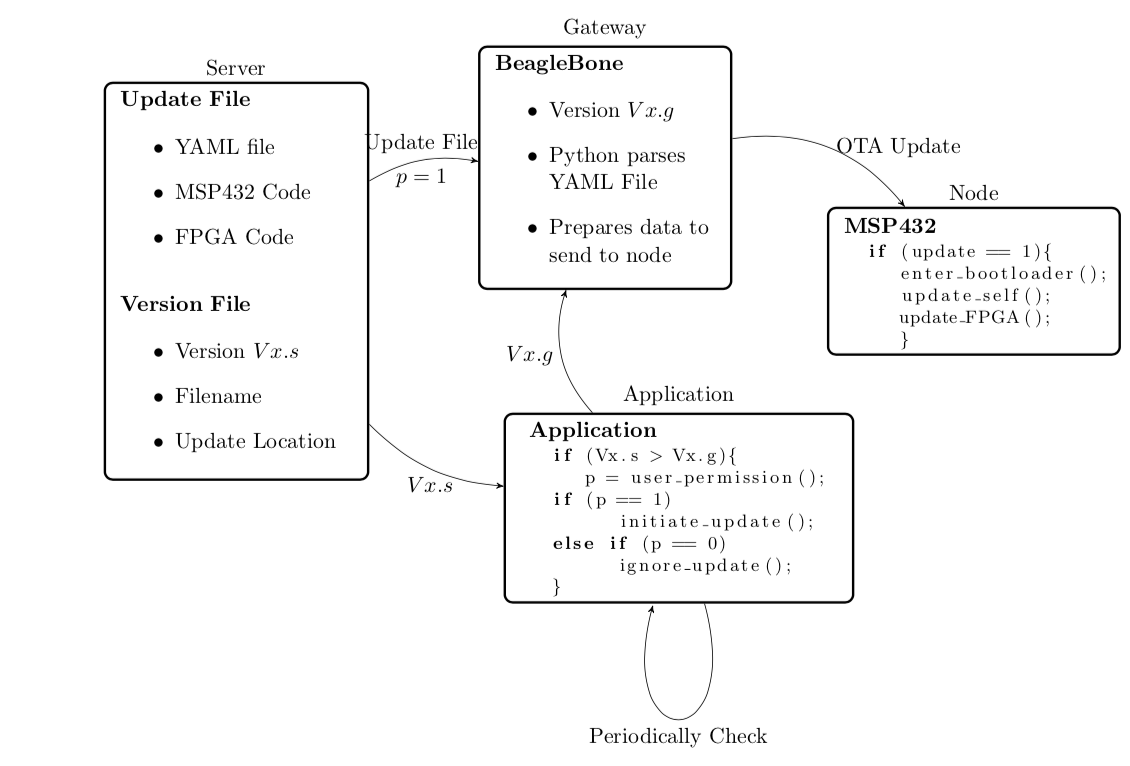
\includegraphics[scale = 0.4]{functional2.png}
\caption{Functional Diagram of OTA Update Implementation}
\end{figure}

}


\section{System Components}


\frame{
\frametitle{Application}
Options:
\begin{enumerate}
\item Check for updates and request update permission
\item Request data from the node (image)
\item Re-Key option from previous project. 
\end{enumerate}
}

\frame{
\frametitle{BeagleBone Black}
\begin{enumerate}
\item Upon receiving update permission, the BeagleBone will download the update file from the external server.
\item The BeagleBone will parse the update information and send the update to the node via XBee. 
\item The BeagleBone will also generate session keys as developed previously.
\end{enumerate}
}

\subsection{Microcontroller}
\frame{
\frametitle{MSP432}
\begin{figure}[!ht]
\centering
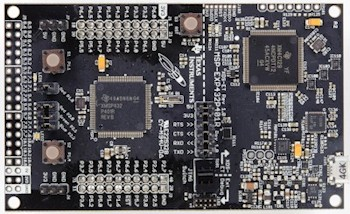
\includegraphics[scale=2]{msp432.jpg}
\caption{MSP432}
\end{figure}
}

\frame{
\frametitle{MSP432}
\begin{itemize}
\item The MSP432 will facilitate communication between all external peripherals on the node (XBee, IGLOO, ArduCam, IR Sensor).
\item The MSP432 can be given a bootloader program which will allow us to access and write to program memory.
\item The MSP432 can also be given STAPL commands to program the FPGA. 
\item We chose the MSP432 because the previous system required enough RAM to handle the transfer of images.
\end{itemize}
}


\subsection{FPGA}
\frame{
\frametitle{Actel IGLOO Nano}
IGLOO nano Low Power Flash FPGA.
Promises revolutionary and leading edge capabilities in less power consumption and smaller size.
Also Allows in system programming using a micro controller (ISP).
\begin{figure}[!ht]
\centering
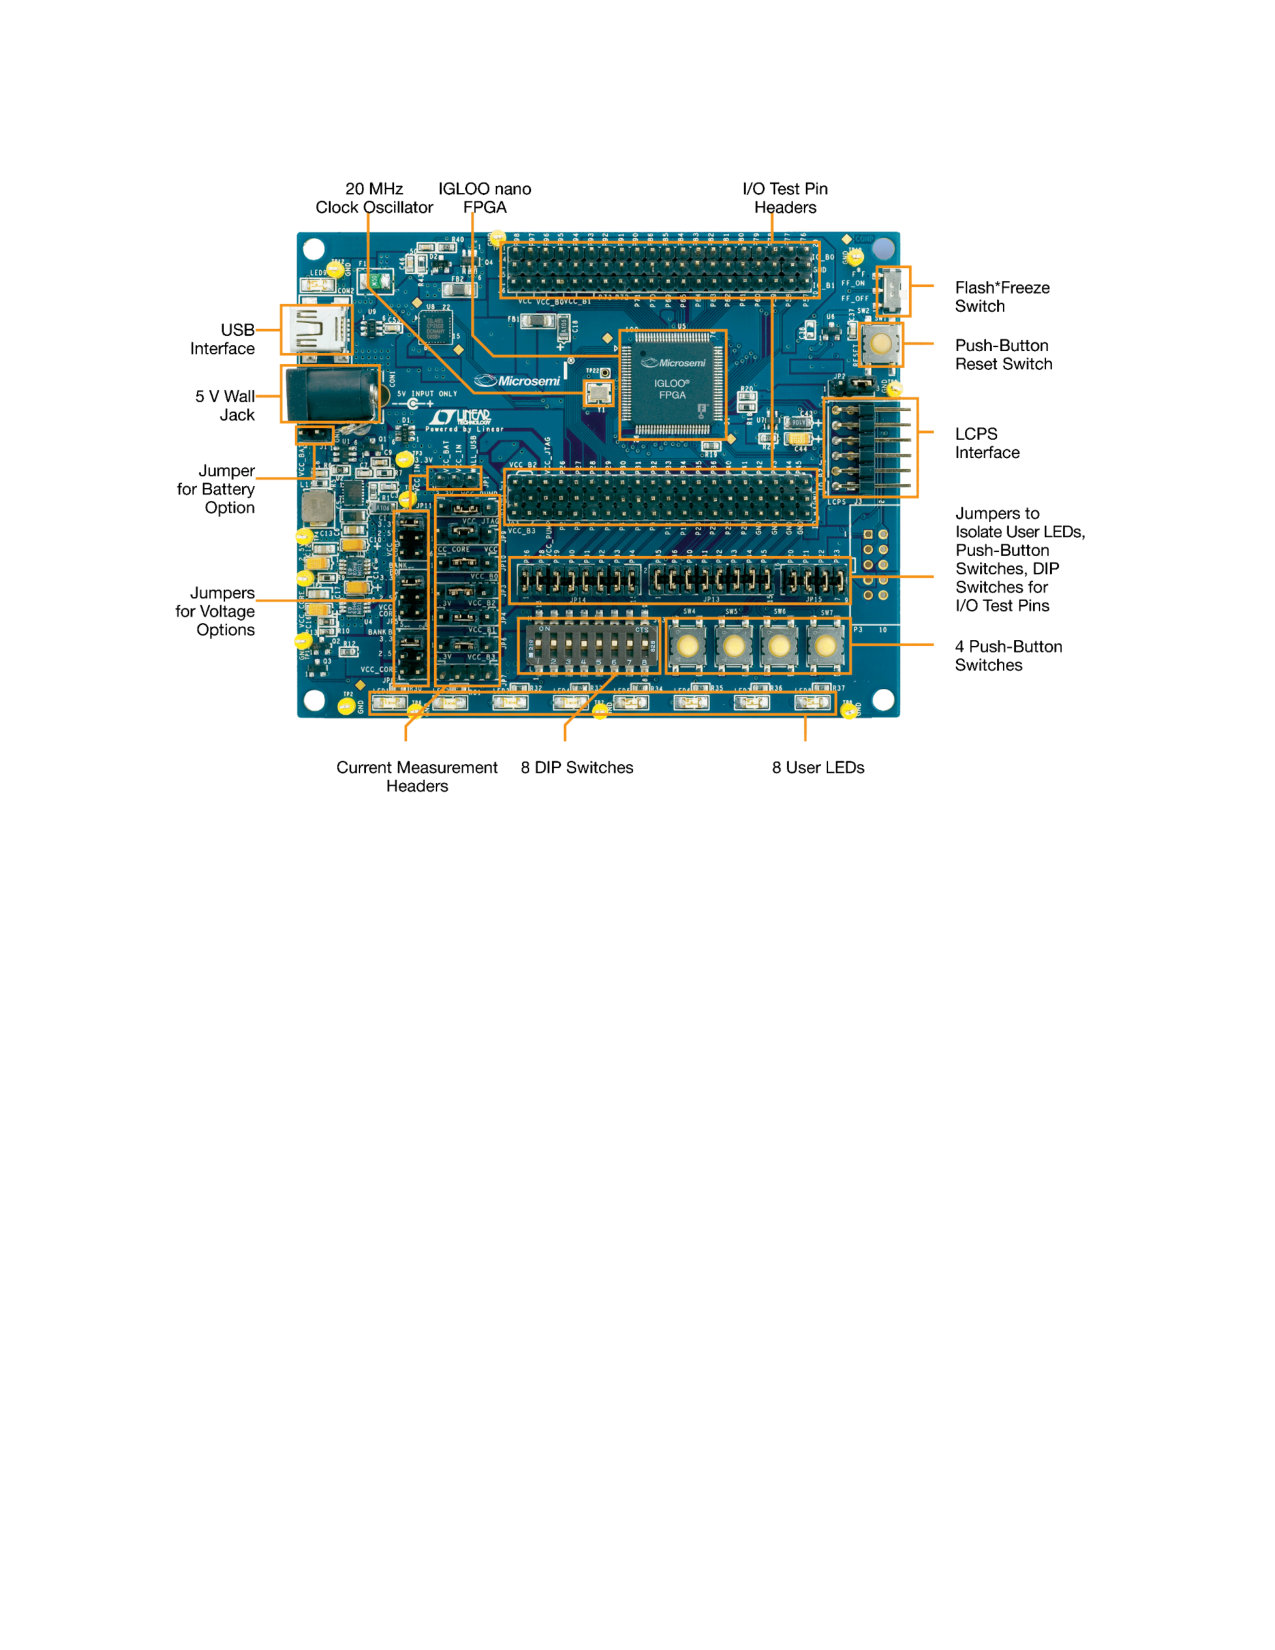
\includegraphics[scale=0.3]{igloo.pdf}
\caption{ACTEL Igloo Nano}
\end{figure}
}


\frame{
\frametitle{Operating Modes}
\begin{figure}[!ht]
\centering
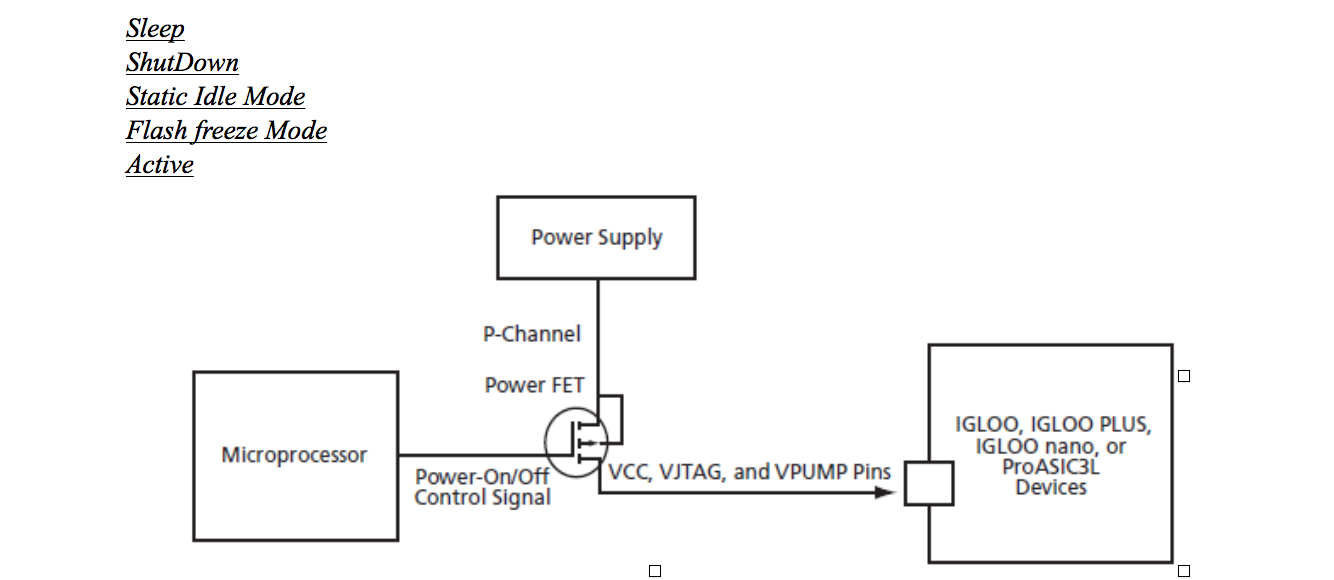
\includegraphics[scale=0.5]{FPGA_Power.png}
\caption{Operating Modes}
\end{figure}
}

\frame{
\frametitle{Flash ROM}
\begin{itemize}
\item The IGLOO nano contains $1\si{kbit}$ of \textit{nonvolatile} Flash ROM memory. 
\item Flash Rom is arranged in 8 banks of 128 bits (128 Bytes).
\item Each bank can be selectively programmed.
\item Flash Rom can be read on Byte boundary 
\end{itemize}
}

\frame{
\frametitle{SRAM}
\begin{itemize}
\item 8 Blocks each of 4,608-bit.  ( Total= 36864 bits or 4.608Bytes).
\item Both the write width and read width for the RAM blocks can be specified independently for SRAM.
\item The read and write clocks are completely independent.
\item 2 synchronous read operations (pipelined and non-pipelined) and 1 write operation for SRAM.
\end{itemize}
}

\frame{
\frametitle{FGPA Programming}
Two ways to program: Device Programming (not used) \\
With Internal System Programming (ISP) (our method)\\
\begin{itemize}
\item JTAG interface on FPGA through JTAG pins. Pins can be controlled by either processor or programmed through a header connection.
\item Both the write width and read width for the RAM blocks can be specified independently for SRAM.
\item It can be programmed repeatedly and erased even if it is mounted. If the
application requires it, the system can be designed to reprogram itself using a microprocessor, without the use of any external programmer.
\end{itemize}
}


\frame{
\frametitle{How to Program}

\begin{itemize}
\small
\item First download the C-based STAPL player or DirectC code from the website.
\item Create the low-level application programming interface (API) to provide the necessary basic functions.
\item These API functions act as the interface between the programming software and the actual hardware.
\item The API is then linked with the STAPL player or DirectC and compiled using the microprocessor's
\item Compiler. (We wont use DirectC since it does not support the upgrading).
\item After compiling download the resulting binary into the MCU system's program memory (such as ROM, EEPROM, or flash).
\item Download Bitstream or STAPL file created using the Microsemi Designer \item software(Libero) into the MCU system's volatile memory.
\item Activate the stored programming binary file.
\end{itemize}
}


\subsection{Updates/YAML}
\frame{
\frametitle{Update}
Updates will consist of:
\begin{enumerate}
\item A YAML file with instructions for the bootloader
\item A section containing the MSP432 update
\item A section containing the IGLOO udpate
\item An update will be initiated by the App
\end{enumerate}
}
\frame{
\frametitle{YAML}
\begin{itemize}
\item YAML is a serialization language that will allow us to map the update to appropriate memory blocks
\item This will allow us to update a specific block of memory at a time.
\item The processing of the YAML file will be done on the BeagleBone.
\end{itemize}
}

\subsubsection{Security}

\frame{
\frametitle{Encryption/Security}
\begin{itemize}
\item OTA update capability can provide a potential vulnerability to the system.
\item We need a system of authenticating updates as to prevent the system using a false update. 
\item We can do this using a digital signature scheme through RSA or ECC. 
\end{itemize} 
}

\subsection{Data Protocols and Memory}
\frame{
\frametitle{Memory}
\begin{itemize}
\item The MSP432 has $64 \si{kB}$ RAM.
\item Both the MSP432 and FPGA have $256 \si{kB}$ of flash memory.
\item The size of the current system is $222 \si{kB}$, and the picture size is a maximum of $60 \si{kB}$
\item In order to be able able to support an update we need to have an external memory pool.
\item The size of MSP432 firmware is $7.5 \si{kB}$ 
\end{itemize}

}

\frame{
\frametitle{Data Protocols}
\begin{itemize}
\item Our wireless sensor node will use the MSP432, which is a low power microcontroller for processing and redirecting sensor data.
\item The FPGA can be made handle the same data protocols as the MSP432 such as $\text{I}^2\text{C}$, SPI, and UART.
\item $\text{I}^2\text{C}$ and UART protocols require 2 pins, while SPI requires 4.
\item $\text{I}^2\text{C}$ and SPI are synchronous transfers, whereas UART is asynchronous and does not require a clock.
\item SPI can transfer at 16Mbps
\item UART can transfer at 960kBps
\end{itemize}
}

\frame{
\frametitle{Zigbee}
\begin{itemize}
\item A high level communication protocol based in IEEE 802.15.4, which is used in low rate wireless personal networks. 
\item ZigBee is common in IoT devices as an alternative to WiFi.
\item This protocol will be implemented using the XBee devices on the Gateway and Node, and will facilitate data transfer between them.
\end{itemize}
}
\frame{
\frametitle{Pros of Zigbee}
\begin{itemize}
\item It is designed for small devices for low power consumption.
\item It is a mesh network standard which can use other devices to pass signals over long distances.
\item The data rates vary from $20 \si{kbps} - 250 \si{kbps}$ in the $2.4 \si{GHz}$ band.
\item Has good performance in environments with low SNR. 
\item Secures data through 128-bit symmetric encryption keys. 
\item Needs less than $64 \si{kb}$ of ROM and $2-32 \si{kb}$ of RAM. 
\end{itemize}
}

\frame{
\frametitle{PCB Design}
For the PCB Design we will need to take into consideration the following:
\begin{itemize}
\item Use KiCad to develop a circuit schematic for the PCB.
\item Redesign the PCB to allow for easier measurement of system specifications such as power consumption.
\item This will require us to fix the previous errors.
\end{itemize}
}


\section{Further Work}

\frame{
\frametitle{Next Steps}
We will need to test each component individually
\begin{enumerate}
\item Getting device to enter bootloader by reading an update sequence
\item Tell the bootloader to write to a specific memory block
\item Begin developing 
\end{enumerate} 
}

\subsection{Experimental Plan}

\frame{
\frametitle{Tests to Run}
\begin{enumerate}
\item We will test our final results by creating an update file, which will call for a noticeable update for both the FPGA and MSP432
\item This update could involve changing the state of an LED.
\end{enumerate} 
}


\section{Task Allocation}

\frame{
\frametitle{Division of Labor}
\textbf{Aneesh}
\begin{itemize}
\item Project manager responsibilities such as keeping everyone on schedule.
\item Create update file, and update verification
\item Work on understanding YAML
\end{itemize}

\textbf{Ryan}
\begin{itemize}
\item Mainly responsible for writing MSP432 code to be able to reprogram itself
\item Working with the MSP432 bootloader.
\end{itemize}
}
\frame{
\frametitle{Division of Labor}
\textbf{Gerson}
\begin{itemize}
\item Create PCB design of final system, for both the gateway and the Node. 
\item Handle any issues interfacing via ZigBee to any of the devices
\end{itemize}
\textbf{Mohamed}
\begin{itemize}
\item Working on the application, which will interface to the server, to communicate with the gateway. 
\item Helping write code to update the BeagleBone on the Gateway
\end{itemize}

\textbf{Sohail}
\begin{itemize}
\item Working on downloading and implementing STAPL player
\item Writing API to be able to interface to the FPGA via JTAG. 
\end{itemize}
}

\section{References}

\frame{
\frametitle{References}

\bibliographystyle{ieeetran}
\bibliography{refs}

}




\end{document}
